
\documentclass[12pt]{report}
\usepackage{geometry}
\geometry{a4paper}
\usepackage{chicago}
\usepackage{makeidx}
\usepackage{tabularx}
\usepackage{graphicx}
\usepackage{color}
\usepackage{pdfpages}
\usepackage{listings}    
\usepackage{float}

\floatstyle{plain}
\newfloat{program}{thp}{lop}
\floatname{program}{Snippet}



\def\keywords{\vspace{.5em}
{\textbf{Keywords} \linebreak \,\relax%
}}
\def\endkeywords{\par}


\begin{document}
\begin{titlepage}
\begin{center}
\lstset{language=Java}  
% Upper part of the page. The '~' is needed because \\
% only works if a paragraph has started.
\textbf{\LARGE The University of Birmingham}\\[0.35cm]
\textbf{\LARGE School of Computer Science}\\[0.35cm]
\textbf{\LARGE MSc in Advanced Computer Science}\\[2.5cm]

\textsc{\Large Second semester mini-project}\\[2.5cm]

% Title

{ \huge \bfseries  Analysing User Interaction On Mobile Devices \\[1cm] }

{\large \textbf{Karthikeya Udupa Kuppar Manjunath}\\[1cm]}

\large{Supervisor: Mirco Musolesi}
% Author and supervisor


\vfill

% Bottom of the page
{\large April 2014}

\end{center}
\end{titlepage}

\begin{abstract}

abstract here.
\linebreak\linebreak\linebreak\linebreak
\begin{center}
\begin{keywords}
keywords here.
\end{keywords}
\end{center}
\end{abstract}


\tableofcontents
\listoffigures
\listoftables
\newpage

\chapter{Introduction}
\noindent
\section{Introduction}
Over the last two decades the world has been revolutionised by technologies beyond what could have been even imagined a century ago. The digital revolution has effected our lives in every possible aspect, mobility is one of the key components of this revolution and has been incorporated in people's live at a very drastic rate [14 -1]. Smart phones and portable devices have become an extension of our persona and have been personalised by us, they reflect our preferences, social choices we make, places we go even the food we prefer to eat. These devices have provided a new meaning to the vision of Mark Wesiser [1] and also a means to achieve more with the growing network of wireless sensors of various kinds in the hands of the people providing realtime information [7]. As we can see in section [x], much work has been done in this direction to make the vision a reality, systems that can provide a groundwork to build ubiquitous systems, algorithms to process the data and make inferences have been developed. This is what we are trying to accomplish in our research as well.

A key component of creating a building block for such a ubiquitous and anticipatory system would be to understand why people perform the actions that they perform at the given time [13] and how it be generalised across the masses which would eventually helps improves their lives without and not be a hindrance, anticipating their actions and adapt itself to their needs [12], Tennehouse [12-43] introduces this concept as proactive computing wherein the system would become so familiar with the user that it would be able to perform action on user's behest.

For us to accomplish this we would need a way in which we can monitor what activities people perform, what are the various contexts which effect these actions and to be able to do this on a large scale. Demographics have been proven to be a very important aspect in extracting features of the user as an individual [12, 4] and also as a collective [6, 3].

This whole process involves a lot of complexities surrounding it, firstly there is an issue of a platform to target, there is also a concern that in achieving such a system we might end up violating user's privacy and interfere in his life all of which among many other are once we address in this research.

\section{Context \& Context-Awareness}
To understand what are the various circumstances under which the user takes a particular action on the device we analyse the \textit{Context} in which the user reacted in the given way. Oxford dictionary defines context as ``the circumstances that form the setting for an event, statement, or idea, and in terms of which it can be fully understood''. Over the years there have been many efforts to define context in terms of computing, [SemI - 30,6,26] all define it in their own way but lack one aspect or the other. In the process that we are doing context would refer to the any information that can define the condition of the user during the interaction between him and the device. This should also cover the relevant state of the device (connectivity, current power level, nearby connected devices among others). [SemI - 8] defines it as``Context is any information that can be used to characterise the situation of an entity. An entity is a person, place, or object that is considered relevant to the interaction between a user and an application, including the user and applications themselves.'' which very clearly defines what our system is trying to accomplish compromising of user, physical, computing and time contexts [SemI -30].

Context Awareness is on the other hand the stepping stone for anticipatory systems. It specifies the ability of the system to firstly know about the state in which it is presently in and eventually adapt itself to the conditions based on its knowledge about the user's preferences. Context-awareness acts as an extension human senses fulfilling its limitation[13] helping in continuously understanding the user's context and improvising itself in its ability to help the user perform his tasks more effectively. Similarly as with all other computing problems, context awareness has moved far ahead from the initial description of context [SemI - 31] with the readily available powerful sensing devices in the hands of masses in the form of mobile phones.


\chapter{Ambient Intelligence \& Anticipatory System}

The field of ambient intelligence and anticipatory systems are closely related to each other, ambient intelligence forms a basis for system which perform anticipatory tasks. Both are a part of what Weiser[x] would have actually thought would come into existence when he said ``The most profound revolutions are not the ones trumpeted by pundits, but those that sneak in when we are not looking''.

The term \textit{Ambient Intelligence} was first introduced in the AmI Challenge in 2001 [E2], wherein it identified AmI at a conceptual level along with components that could be developed to make this a reality. [E3] defines it as an environment wherein the the environment would adapt itself to the needs of the user, there would be a lack of any input devices to take user's feedback instead there would be sensors which would blend in into the environment's day to day items, connect with each other and constantly try to adapt themselves and improve the life of the user. Anticipatory systems as described by [E5] is ``a system containing a predictive model of itself and/or of its environment, which allows it to state at an instant in accord with the model's predictions pertaining to a later instant". Hence, the system itself has to be intelligent enough to make predictions about the future and adapt itself which makes it very similar to ambient intelligence, difference being the ambience of the technology which may or may not be there in the anticipatory system. The current framework and application mentioned further in this report form the ground work for a system which falls into the category of both ambient intelligence and anticipatory system.

\section{Components Of Anticipatory System}
An anticipatory system has multiple components which work together to provide the desired results. As we have seen context forms an essential part of any system that deals with understanding and improving user's day to day tasks and habits. Majority of the information required to do such a task is extracted from the sensors that are available in the devices, however the data as is useless and also usually limited to a single user. We require a larger dataset of multiple individuals that can then be used alongside machine learning algorithms to develop a model and extract meaningful inferences. These inferences can then be used to predict future events and gradually improve itself and its prediction over a period of time in the form of reinforced learning. This process, [E1] categorises into four stages:

\begin{itemize}
\item Sensing of the contextual information of the user.
\item Extraction of feature from data.
\item From the available data make predictions for/about the user.
\item Understand its mistakes and improvise itself to provide more accurate and useful information.
\end{itemize}

Let us further look into each of the above mentioned step in depth.

\subsection{Sensing}
First and foremost step in any anticipatory system is to collect information about its users. The information is usually quasi-continuos sensor reading from the device's various sensors [14] and other similar contextual data that we can gather about the user. The amount and kind of data varies on various factors such as the availability of sensors, portability of the devices and the actual requirement of the system.

With the advent of modern mobile devices we have a plethora of sensors encompassed in a single device which the user is almost certain to carry around and use continuously. This presents an opportunity to for us to extract meaningful information about the user in his natural environment without actually interrupting or obstructing his day to day tasks and without him deviating from his natural flow of work. Almost every smartphone these days has basic sensors such a GPS. accelerometer, light sensors among other and can usually connect to the internet [Diagram 1]. This provides us with a very rich source of contextual information which we can harness for gathering data about the user. This is not just restricted to mobile smartphones but can be extended to various other platforms such as music players (iPod's), tablets, gaming consoles (XBOX, Wii, Playstation), home theatre systems, vehicle GPS navigations and many other components that we interact with almost every day, all of which provide some source of context which we can use.

All the data that was discussed above refers to a person's individual information and is usually referred to as \textit{Personal Sensing}[E7] but with the recent growth in mobile internet networks, people are always connected and so are the devices to both each other and to the web this allows us to not only sense the information but also to provide it onto a central location on the worldwide web. However on a larger scale where we are monitoring a group of individual or a community of people to identify patterns and emerging trends, this is termed as \textit{Crowd-sensing} where in individual's devices collectively provide data to identify phenomena's of collective value to the community [E6]. There are already several real world examples which use community based sensing in areas like environmental monitoring[E6 - 3] and navigation[E6 - 4/5], the only shortcoming of this being unable to interact with the test users personally and take their feedback which can be done with personal sensing.

[Diagram - iOS Context -
- Accelerometer, Gyroscope, Proximity, Ambient Light, Magnetometer, GPS, Bluetooth, Microphone, Fingerprint, Camera, Moisture Sensor

S5 Context - NFC
]

Although sensing, both in terms of personal or community based seems very promising and can provide much in building better systems but are not without their issues and drawbacks. The availability of the data is very much platform dependent, with multiple devices and mobile operating systems deployment is one of the key challenges along with the issues faced on each of the platforms. Additionally as it is with all researches which makes use of user's information privacy of the user and his information is a key concern. We will discuss this further in section \ref{challenges}.

\subsection{Feature Extraction \& Context Association}
The raw sensing data acquired from the sensors whether locally or remotely in the case of crowd-sensing is not of much use to us as raw data itself contains lot of noise, we need to interpret the raw data to extract relevant features based on our requirement. For example we can have the raw data from the accelerometers how do we understand from the accelerometer x,y and z the activity of the user [E8], or maybe the mode of transport which is using at present or if he is just sitting at his house, if the user can be interrupted at a point in time [Intrup Print.]. There are various platforms and statistical tools readily available for each of the data stream. However each data stream might be used to extract different characteristics [E1], for example sound can be used to identify the present surroundings of the user however it can also be used to understand the physiological state of the user as well. So the feature extraction actually depends on what you want to do with the data available.

Another challenge is with crowd-sensing and global distribution pattern using Google Play Store and Apple iTunes store the application usage and in turn the data being gathered can scale at an immense scale. One way to reduce the problem is by removing context information that is of not related or can be ignored, this helps by reducing the load and also by cancelling the negative impact on the results.[12] 

Additionally, there are other co-context's that can be fetched using the available context context information. For example, if our application has some relation to the location of the place the user is in, weather becomes a co-context which can be found with the help of the location context. Similarly, if location itself is not directly available but we have GPS or WiFi information we can calculate the location from it.

\subsection{Anticipations}
Understanding the features and extracting the information from the sensor data provides us with an opportunity to use this information for much more then understanding the present context of the user. By knowing what user's choices are we can make predictions for the future.

From the extracted features various supervised learning models can be constructed which can associate user's activities and the related context. This when applied to the collective data of the community helps us build an effective model which can help us anticipate things for the user both as an individual and for the community.


\subsection{Improvement and Self-Learning}


\section{Components of the present systems and how it related to anticipatory system}

The system in question is a foundation of an anticipatory system, to understand how the system works as an anticipatory systems we need to understand the various components which interact with each other and other components that can be linked with it to make it a complete anticipatory system. The system presently is build for Android mobile platform and supports devices running Android OS.

The primary component of the the system is to gather information for further processing. This task is performed using the context sensing framework, which provides all the context information based on subscriptions. Other then context, user's application usage is also one of the most vital component of the system. This is extracted from the mobile's default API. The framework and the sensing process and strategies are explained in further detail in section [x].

Since the application falls in the category of crowd-sensing, the data is sent to a central data store on the web from the various devices of individuals. The application makes sure that the data is sent to the server in a power and money efficient manner (See section [y]). The server is responsible for storing the information securely and also acts as an authentication server. Essential features are filtered and context is associate with each other and the user. Further also tries to understand the extracted information and provide end points for the application to get prediction data and analytics information (See section [z]).


\chapter{Context Sensing Framework}
\label{ContextSensingFramework}
Context is a very primal component of any system. As seen in figure 1, the contextual information provided by modern smartphones is enormous. However, the mobile platforms are various and each platform has its own development environment and is different from one another. We selected the Android development environment for the study as this provides a much more flexible and open framework to extract contextual information then its Apple iOS counterpart [E9], which restricts access of information for an application beyond its application sandbox and also restricts it from collecting information in the background.

Although there have been many contextual frameworks for Android which provide an relatively easy methodology to extract information [E10, Print 1], however the present requirement is rather simpler and there are some components that the framework does not monitor, for example, [Print 1] does not matter network, WiFi access points, [E10] does not monitor user's schedule among others.

The context sensing framework designed for this purpose provides a very interface to connect to application for any purpose.

\section{Types of Sensing}
\label{contextType}
There are various sensors that can be selected to be monitored by the framework on Android, the following information was considered to be monitored for the first version of the framework.

\begin{itemize}
\item Location (GPS or Network)
\item Battery/Power Source Information
\item Network Connectivity
\item Network Signals
\item WiFi Access Points and Connectivity
\item User Events
\item Bluetooth Status and Nearby Devices
\item Telephony
\item Screen Activity Context
\end{itemize}

We will further discuss each of the the above mentioned context's in details and how a scanning methodology was customised for it making effective and efficient.
 
\section{Framework's Working Architecture}
\subsection{End-points and External Handling}
\label{ExternalHandling}
The primary objective of the framework is to make sure information is provided in the simplest possible way and can be customised accordingly. Also the framework has to be plug and play, meaning there should be a minimal lines of code that requires to be added to an existing application to do what you want to do. The functionality of any existing application should not be focused on getting the framework to work but rather framework should just be a component integrated into the application providing a stream of required information and can be controlled effectively. 

The architecture of the framework that was designed can be described as a subscription based model, wherein each of the components can be subscribed externally. In addition to that each subscription can be provided with parameters to customise it.

To begin monitoring any particular context one just has to call the \textit{monitorContext} method in the \textit{ContextManager} class. The call can be customised by the parameters that it accepts.

\begin{program}
  \begin{verbatim}

public void monitorContext (
            ContextManagerServices mService,
            long minimumUpdateTime,
            long pollingTime,
            ArrayList<Integer> flags
    );
\end{verbatim}
\label{monitorContextCall}
\caption{Function definition of the monitor context.}
\end{program}

As we can see in the function call, there are several parameters, let's look into them for more detailed understanding.

\begin{itemize}
\item \textbf{\textit{ContextManagerServices} Parameter - } \textit{ContextManagerServices} is a enumeration defining various types of context's that can be monitored by the framework (see appendix 1), this specifies which of the context's the application wants to monitor using the framework.
\item \textbf{\textit{minimumUpdateTime} Parameter - } This specifies the minimum time the application should receive an update about the specific context regardless of if any change has occurred or not, this is useful for application which want information about context at regular intervals to update their UI or other purposes.

\item \textbf{\textit{pollingTime} Parameter - } This parameter specifies the time interval after which the framework should poll the sensors or the operating system for information about the context. This parameter is particularly useful for information which do not have system provided callbacks (Broadcast/Intent architecture) and require polling or cases where power consumption for constant monitoring is steep and is not feasible.

\item \textbf{\textit{flags} Parameter - } This is an extensible parameter which is essentially an array of flags which can be passed to the framework. This also allows for easy extension to the framework without much change in the call in the future. An example for the use of the parameter is for passing information about the source to use for location tracking.

\end{itemize}

With this call one could essentially start monitoring any context that is available in the framework. Another requirement for an effective framework is to be able to deliver information to the specific application. In case of the parameters not provided the framework automatically allocates a default timing specific to the intent.

[Figure 2 - Broadcast Intent Reciever Arch.]

Android provides a very effective methodology to transfer information between objects called Broadcast and Intent receiver architecture [E11, E12]. The working of the methodology is very simple yet very effective. As [Figure 2] explains we can ask for an object to register itself to the \textit{LocalBroadcastManager} to be notified in case it receives a broadcast with a particular name or tag which is referred to as \textit{action} in android.

The framework harnesses the power of this methodology in Android to provide a single point receiver to all contexts. 
[Figure 3 - Framework Architecture]

The application would have to register just once to the\textit{LocalBroadcastManager} for any and all context's it is monitoring. When the framework has an update it would send a broadcast, which would have the following components:
\begin{itemize}
\item \textbf{Action - } All broadcasts from the application are associated with one action string `\textit{CONTEXT\_CHANGE\_NOTIFY}' regardless what type of context it is.
\item \textbf{Additional Information - } Other then the action, broadcast can also contain addtional information in the form of a key/value pairs. The framework sends various other values for each broadcast.
    \begin{itemize}
    \item \textit{CONTEXT\_TYPE - }The type of context the broadcast contains. [See appendix 2 for detailed list.]
    \item \textit{Context Information Flag - }This flag is named after the context type that is passed, hence varies depending on the content it contains, the value is a JSON (\textit{JavaScript Object Notation}) formatted string containing information passed by the framework.
    \end{itemize}
\end{itemize}

Finally, the application should be able to stop monitoring a context as easily as it begin monitoring the context. The context can be stopped from being monitored and hence the application would receive no further updates by simply calling

\begin{program}
  \begin{verbatim}

public void stopMonitoringContext(
            ContextManagerServices mService
        );
\end{verbatim}
\label{monitorContextStopCall}
\caption{Function definition to stop monitor context.}
\end{program}

\subsection{Internal Working}
The internal working of the framework relies on multiple components of the framework interacting with each other. As described in section \ref{ExternalHandling}, \textit{ContextManager} is the external interface with which any application trying to use the framework would interact with. The class is also responsible for delivering broadcast at \textit{minimumUpdateTime} intervals. However, the framework works on a set of classes which ensure that latest information is always available and done effectively.

A singleton class, \textit{ContextMonitor} is primarily responsible for performing monitoring at the given time intervals and updating the context values for the \textit{ContextManager} to use. There are two kinds of contexts that we have to deal with.

\begin{itemize}
\item \textbf{Polling Tasks - } Certain contexts need to be accessed using Android system API calls at the required time intervals, for this the we use a timer task in \textit{ContextMonitor} is initialised to do the polling task for it. In case there is an update in the information a broadcast is sent to all listeners about it.

\item \textbf{Monitoring Tasks - } Some of the available contexts have a broadcast and intent model provided by the system itself, so in this case, a broadcast receiver object for that particular action is created in the singleton to receive information and update its variables accordingly and in case of a relevant change a broadcast is sent to the receivers.

There are several advantages of using the development model, primarily this provides a single point of access to all the information that is required by the framework which in itself is very beneficial in scaling the framework further. Additionally, a single instance of the monitoring task ensures there are no multiple tasks being run by the framework in case the application using the framework starts to monitor same context at multiple places. Although, this might look very minimal but for polling tasks like location information and bluetooth scanning this is very effective in terms of resources spent.

\end{itemize}


\section{Understanding individual context monitoring}
Each of the context's being monitored by framework have their own unique methodology in which they work. The uniqueness helps them to perform monitoring in a very effective and power efficient way. Let us look in details a two of the important context's working.

\subsection{Location}
Location, one of the most important contextual information that can be extracted. With modern devices which people carry everywhere it has become all the more important. The major concern with location is the power consumption factor when using GPS [E14], so constant monitoring of GPS is never recommended on mobile devices. Also, time it requires to switch on the GPS sensor and get a triangulation from the satellites can also be a concerning factor sometimes. Modern devices provide network based location services which require both network connectivity and internet to provide location. This process is battery efficient but accuracy is usually questionable. 

The framework provides the application option to opt for either of the technique in addition to the ability to specify the polling interval.

[Figure 4 - Location Working]

Android operating system itself stores the last known position [E16] which is updated when any of the application triggers the location manager. So at the given polling interval the device first looks for location by using the \textit{getLastKnownLocation} method. Then the system analsyes if the location that is been provided by the system is a better location then the one it already has and if it meets the criteria (freshness of the location), if the criteria is met this location is stored and broadcasted. If not, the system would trigger the specified location provider (GPS or Network) to provide it with a new location, the fetched location is then broadcasted and stored.

\subsection{Network Information}
Mobile phones are usually connected to networks, when the user moves the connection to the network also changes. The systems decides which signal providing tower to connect to out of the ones that are available. This information can be very useful in terms of context. For example with this information one can map the network density and signal strength of the area. There are several components that constitute of network information and there is not a single method to monitor this.

[Figure 5 - Network Working]

\begin{itemize}
\item \textbf{Signal Strength - } Signal Strength constantly changes and can be monitored by a system provided broadcast receiver. However the frequency of the change is very high, hence broadcast is done only when there is a significant change.

\item \textbf{Cell Towers Nearby - } Although the device usually connects to a single cell tower but there are various other towers which broadcast their presence and the device picks it up along with other information such as their signal strength. This information is also provided through a broadcast receiver by the system.

\item \textbf{Data Connectivity - } The networks may or may not be providing data connectivity to the device or the user might have turned off the data connectivity. This information needs to be polled constantly as the broadcasts are not reliable and do not provide internet connectivity information. The framework frequently checks for updates about connectivity information and notifies if there is any change.

\end{itemize}

\section{Shortcomings \& Possible Improvements}
\label{contextShortcomings}
The framework provides a foundation for a much more extensible and useful framework for android. There are several areas which should be considered in the future versions and will improve it further.

Firstly, the framework can be made more robust, currently it has been designed for devices running Android version 4.0 and 4.4, backward compatibility would certainly make the framework useable on a wide range of devices. 

Although android is at present one of the most popular operating system in the mobile arena, there are a considerable number of the mobile users who use other popular operating systems like iOS and Windows platform, an extension of the sensing framework with similar functionality (within the bounds of the operating system) on other platforms would be certainly helpful in conducting studies with a broader group of audience then just people using android.

Additional context's like accelerometer and application monitoring (currently implemented in an external app using the framework) are presently missing in the framework and would be a valuable addition to it.

The sensor information gathering technique is primal in nature and lacks adaptive qualities like in EmotionSense [E10], which allows the sensing to be done adaptively instead on a fixed interval. For example movement of the user should be tracked based on the movement he has done during the last interval, if the location change between two interval is considerable less or none, the next sensing should take place an increased interval or if the change is considerable the sensing time interval should be reduced. Additionally, it should take into consideration the battery usage of the sensor and the current state of the device, i.e. sensing intervals should adapt itself based on the battery life of the device.

Given enough time the framework can be expanded into a much more robust, functionally rich and highly customisable component which can be used in various kinds of studies and real world application. 

\chapter{User Demographics Data Collection Application}
The primary purpose of this project is to collect information about how the user interacts with his mobile device, the framework provides a foundation through which we can collect information about the contexts in which the user is using the device, but presently does not provide information about how the user interacts with the device's application and uses websites.

The \textit{WebSense} application was designed for Android platform for the very purpose of collection of user app usage demographic collection along with contextual information. The application integrates with the context sensing framework described in chapter \ref{ContextSensingFramework} to extract contextual information of the user from the device.

There are two aspects of the application which were taken into consideration while designing the application. First was the actual development and effective technique that was to be used to monitor how the user interacts with the device, second is the value it provides to the user which should be lucrative enough for people to install even if they are not interested in the research value of the application.

\section{Application Usage Demographics Collection}

Android is a very open platform in terms of providing data when we compare it with the next most popular operating system for mobile iOS, which restricts application in a sandbox [E9]. This allows us to monitor various minute details about user's smartphone interaction.

The most essential requirement of any such application is to be able to make sure that it has an almost 100\% uptime, meaning it should be always running in the background and performing its tasks. A front end application provides user an option to terminate the process very easily by accident hence denying the change of gather information. However a background service on the other hand is usually not that easy to be terminated and does not hinder the user's mobile phone usage.

The application consists of several of background services each with their own tasks. 
\subsection{Application Usage Monitor}
The first and foremost one is to monitor the user's application usage dedicatedly. This is done by the Service called \textit{AppUsageMonitor}. The service is a self-reviving service so in case it is terminated or malfunctions it revives itself, ensuring almost an 100\% uptime.

Android provides an access to the currently active tasks with the \textit{ActivityManager} framework. The framework not only provides with the running tasks but provides it in the order of its screen presence, meaning using this information we can identify which application is currently running on the screen of the user and is interacting with. However as this is a polling tasks it has to be done very frequently to collect accurate information.

Additionally, android also provides intents which one can listen to for detecting user's action of switching screen on and off, which in-turn means we can safely stop monitoring user's activity tasks when the phone is turned off hence saving crucial resources. 

The application stores the information in a SQLite database, this includes package name of the application, start time, end time (Both in UTC timestamp format), duration of the run, location it was used at (subscribes to the framework, listens and stores location information constantly) along with the day of the hour the application was used at. Additionally, a flag marking the synchronisation state of the record is also maintained. Whenever an application switch is performed the data is written into the database hence minimising the chances of data loose incase of a malfunction or termination. A save is also performed in the scenario when location update is received while an application is running, hence there would be multiple instances of a constant application session if the user is moving. This is particularly useful in case of navigational applications.

If the application is the default browser of the device, the app also detects the page user is viewing. Although, there is no direct way to perform this, android provides an API to access browser history [E17], the topmost object being the current page the user is viewing. Whenever user changes the webpage a new record is created and the time spent on the particular webpage is noted.

\subsection{Contextual Information Monitoring}
\textit{ContextBackgroundMonitor} class is also a background service which is responsible for registering and monitoring the contextual information. Presently it monitors all the contexts provided by the framework (see section \ref{contextType}). Its responsibility is to make sure that as soon as the service is initiated it subscribes to context information broadcast and whenever there is a message it saves it appropriately in the database. Since we are focusing on location for mapping the information and also providing user with information in relation to his location, all the context information is stored with the latest location information.

The class is initiated as soon as the monitoring begins and when the class is destroyed it releases all the receivers and initiates the stop procedure in the framework (see section \ref{ExternalHandling}) hence stopping monitoring process altogether.

\subsection{Web Synchronisation Service}
The sensing and the app monitoring generates a lot of content which then is stored in the database. This can be used for local analytics (see section [X]) but this application is a crowd-sensing application, meaning we are to analyse information of all the user as a collective. For this purpose, the information that is in the device has to be constantly sent to the server.

\textit{SyncManager} is the class responsible for synchronisation of the location content on the web. After a fixed interval the class is revived (if running only \textit{onCreate} is called) and it checks for records which have not been synced in the database. To avoid repetitive reads the monitoring services automatically increment count and store it on a preference file. If the criteria for data upload is met the information is uploaded in chunks of fixed size in the form of a JSON string and as soon as the data is successfully uploaded the records are marked as synced. The synchronising process users the end points provided by the web application and sends the data after compressing it with gzip [E18]. The records are sent with an authentication key to both validate and associate the records, this key is obtained during the login process [see section x and y].
[Sync process algo - Criteria]
The service is also responsible for periodically clearing old data which has been synced already and are outside the time-period in which they could be useful locally (30 days in this case).

\section{User Interface \& Application Value}
The purpose of the application is to collect data not only from people who participate in the research but from as many android user's possible. As previously conducted studies have shown that one of main issue when dealing with crowd-sensing application is that it is bottle-necked by the fact the whole research and the application's success and the amount of data gathered depends on the sole decision of the user to install and keep the application on his phone [ref demographics paper]. So to ensure people install and keep the application we need to provide the user some utility value through the application.

The user interface of the application which runs atop the data gathering services provides some feedback to the user and also helps in collecting some user related information.

\subsection{Login interface}

The login interface is the initial screen of the application where in the user provides the below mentioned information if he is registering or just logs into the application if he has already registered.
\begin{itemize}
\item Email Address
\item Password (For associating records on multiple devices using same email.)
\item Gender (Provides a feature to use in classification.)
\item Employment Status (Additional parameter, which can be used in learning algorithms to verify information extracted from patterns)
\item Consent to allow monitoring (along with a link to the End user's license agreement)
\end{itemize}

An option to log out of the application is also provided inside the application, in case the user wants to stop the monitoring or wants to do something privately.


\subsection{Application Usage Information}

The usage of the various applications which is being constantly tracked by the background monitoring services is provided to the user in the very clean and minimalist user interface along with an option to filter the information to a particular duration (day, week and month).

This information is extracted from the devices local information database, by aggregating the overall usage of each of the application.

\subsection{Application Usage Trends}

This provides similar information but instead of providing information for user's application usage, it provides aggregated information about all the user's using the application. It shows the trends of application usage based on the data accumulated. The web API has an end point which provides the information for the duration required for (day, week or month).

The application's information is also provided along side, hence icon and the name of the application is shown along with an option to install the application if it is not already installed.

\subsection{Web Usage Trends}

Along with the application usage trends the app also shows information about the web usage trends, showing information along with some content and images from the websites popular among the masses in the given duration.


\subsection{Localised Web and App Usage Trends}

The information about the app and web is also provided for a limited geographical area, meaning the app provides what is popular in the user's current area. This can be very helpful for example, if the user is opens the application at a train station the app would provide information about the apps and websites people use there, which are most likely to be the ones providing information about the the timings of the train.

The geographical radius is decided on the server the location is provided by the context sensing framework which then is passed along with the web request. The process of handling this request is discussed further in section [x].

\section{Web API and Feature Extraction}
The application provides a very robust way to gather information about the user and also to do some local analytics and processing for him to show his usage trends. However, to provide information for a community the application has to analyse data not just from a single user but from all the users using the application. This can be done with a web application capable of receiving information, saving it, processing it, extracting relevant information and providing useful information and maybe even do prediction.

A web application was build and deployed on the internet for this purpose. The application is build using Node.JS [E19] which provides a very strong foundation to build high performance web api's and application which have to deal with an increasing number of web requests [e20]. The backend for the application is a MongoDB non-relational document based database [e21] which provides various functionalities to process and extract information along with a lot of scope to improve the performance and handle scaling of the web application.

The web app is essentially a collections of RESTful API end points with JSON data format to store, process and display/provide information. Let us briefly go through the available api's and how they work. All the service accept gzip request to enable minimal data usage. The server is presently hosted on an Amazon EC2 instance of a minimal size.

\subsection{Storing Information}

The application stores various types of information. The first and foremost request the app makes is to register or login, the information about the user is stored in the \textit{user} collection. The user document is designed to handle multiple devices and multiple sessions running simultaneously, the document model also stores other information that is sent by the app when the user registered.

When authenticated the service checks for the user record along with the device information and either creates or updates the device information that is provided with the login information and returns a unique authentication key which can be used for all further requests.

Storing of web and app usage information is more complex, when the service is called the first thing the server checks is if it is a valid service in terms of the authentication key that is being supplied. If it is, then it starts processing the information that is provided. The user is almost instantly provided a OK status message while the processing is going on.

[Figure app processing information]

 It collects all the package names that were sent in the requests and checks the existing database of application information for their records, the ones which are new are then sent to a different service call which asynchronously checks each of the package name and fetches information about the application from the app store by scrapping the web page for information.
 
The location information is also corrected and stored in the required format to perform geospatial queries later on.

The process for storing context information is also identical, except there is not much processing at present.

\subsection{Extracting meaningful information and patterns}

The web app is also responsible to identify and provide patterns to the application on the device about application and web usage. The information is extracted from the database using the MapReduce technique which MongoDb supports. 

The process for extraction of information usually involves aggregating the app usage for each package, however,this can also accommodate things like duration and location information. Location filtering uses the geospatial functions that is provided by mongoDB to reduce the records to a particular area only. The radius along with things such as packages to ignore can all be configured in the config file. The diagram above shows in depth the working of these queries.

\section{Possible Improvements}

The application and the framework was both developed over a period of 1.5 months. The purpose of this project was to create a foundation for a robust data collection application and a framework which would be re-useable component for context extraction. This being said, there are various improvements that can be done the application and the web application.

\subsection{Android App Shortcomings  and Improvement}

The android application lacks several features in this first release. Firstly, improvements that were mentioned related to the framework (see section \ref{contextShortcomings}) would improve the overall performance of the app.

The application presently provides analytics and trends information which is very generic which can be customised and converted to a very personalised recommendation system (see section \ref{RecommendationSystem}).

\subsection{Web App Improvement}

The web component can be improved considerably both in terms of features that it provides and in terms of performance. 

\begin{itemize}

\item Presently there is no web front end for the analysis of the information that is being gathered, only way to access and analyse the information is by directly accessing the information though the database.

\item The web component at present does not deal much with the context information, it just uses app usage and location information to provide the various results, future improvement can make use of all the available information. 

\item The web component's security can be improved by using bcrypt to store and encrypt private information.

\item The database connection at present picks a connection from a pool of 10 connections. There are several things that can be done to allow fast network transactions.
    \begin{itemize}
        \item Sharding [E23] maybe applied and to the mongodb instance to improve the performance of the application.
        \item At present the application relies on mongodb to deliver it data, which in turn reads from the database and provides the required data. With the increasing load this would not be feasible. A caching layer which would store the information in memory would be required. Technologies which are meant to handle rapidly changing content in the memory such as Redis can be used for this purpose in the future.
        
        
        \item Use of MapReduce technique to perform various complex functions in the application benefits the overall performance, but at present each time the service is called the MapReduce is performed. This can be avoided by using incremental MapReduce [E24] which automatically reduces the information when new information is added incrementally hence reducing the load on the server by a considerable amount.
    \end{itemize}

\end{itemize}



\chapter{What can be done with the data}
The purpose of this stage of the experiment is to provide an effective way to gather information from the user at a very large scale. Presently this information is being stored and analysed to provide statistics and trends in a particular area and the user community. But there is much more that can be done with the application.

Let us look at a few possible novel approaches to use the information that has been gathered in future researches.


\section{Intuitive Application Launcher}

A very simple application on the lines of [ref. falcon paper] and which we are already working on would be to build an intuitive launcher based on the information that has been gathered. However, rather then actually launching the application we can provide a much more simplified approach.

[Figure idea screenshot]

On switching on the screen the application would present the user with options on the lock screen itself to launch application, the list of application for the user to choose from without opening the application list, this kind of predictive computing can be very helpful for the user and save him from searching for the application.

We already have contextual information about the user and the app usage, we would require a combination of both web and local processing to actually provide the options.

Additionally, this system can learn based on the choices user makes on the launch screen, whether or not he selects one of the app provided and eventually improve itself.

\section{Recommendation System}
\label{RecommendationSystem}
The application already uses the existing information available to provide recommendations as per trends but this functionality can be extended further, presently the app gives a very generic recommendation both for overall user-base and location specific recommendations, but improvements can be made to recommend people what to use based on their specific usage trends, for example if a person uses a certain application for ordering food however there is another app which is popular in his region (making an assumption it might actually be better the the one user has more relevant results for his location) the application can make a suggestion to the user to try out the application.

Similar functionality can also be developed for web pages, a recommended reading list can be formulated based on the user's reading habits and the trends, this would require a natural language processing of the content of the webpages to understand the nature of the content on the website. The application would have to understand the user's web usage pattern and derive a web profile for the user and improving over a period of time. This would be similar to [E22] but for mobile devices hence would be able to learn and adapt faster, also since the content which is recommended is already popular among people the possibility of a favourable recommendation is more likely.


\section{Pre-Caching}
We can use the information acquired from the gathered data about popularity of applications at certain location and time along with information about user's preferences to intelligently launch application in the background or to load content on to the devices locally beforehand hence reducing the wait time for the user.

Additionally, this can be converted and expanded into a much larger framework. We could use the information from the server and transfer into local WiFi access points, which can then use the web usage information and intelligently cache websites/webpages which are popular in the vicinity of the access points. This would require an integration of the server and the WiFi access point. This would provide a very large scale increase in the speed by which the popular websites are loaded on the mobile device hence providing a much more smoother experience. However, this process has to be designed intelligently else it can result in providing stale information to the user.


\chapter{Performance Evaluation}
\chapter{Challenges \& Downfalls}
\label{challenges}
\subsection{Deployment \& Platform Restrictions}
The present application is meant to be used only with Android operating system, this restricts the users with other devices to participate in the stay and moreover hamper overall demographics of the study, even though [e25] shows that android has a majority in mobile marketshare there is still a considerable number of user's using other operating systems and also this figure can vary based on the location where the survey is conducted, hence making it very important to conduct the study on a broader scale.

However, lot of what is possible would not be possible on operating systems such as iOS. iOS is governed by a sandbox policy [E9] which does not allow to access information (such as application on top) other then its own.

\subsection{Data privacy concerns}
\subsection{Accident Behaviour Modification}
\chapter{Related Work}
\chapter{Future Work}
\chapter{Conclusion}
Practical usage of the information as we have seen is a lot, however, this information can also understand various aspects of people and mobile phone usage behaviour in a better way.


\bibliographystyle{ abbrv}
\bibliography{mini_project_report}

%APPENDICES
\appendix
%Mini-project declaration
%\clearpage
\chapter{Mini-Project Declaration}
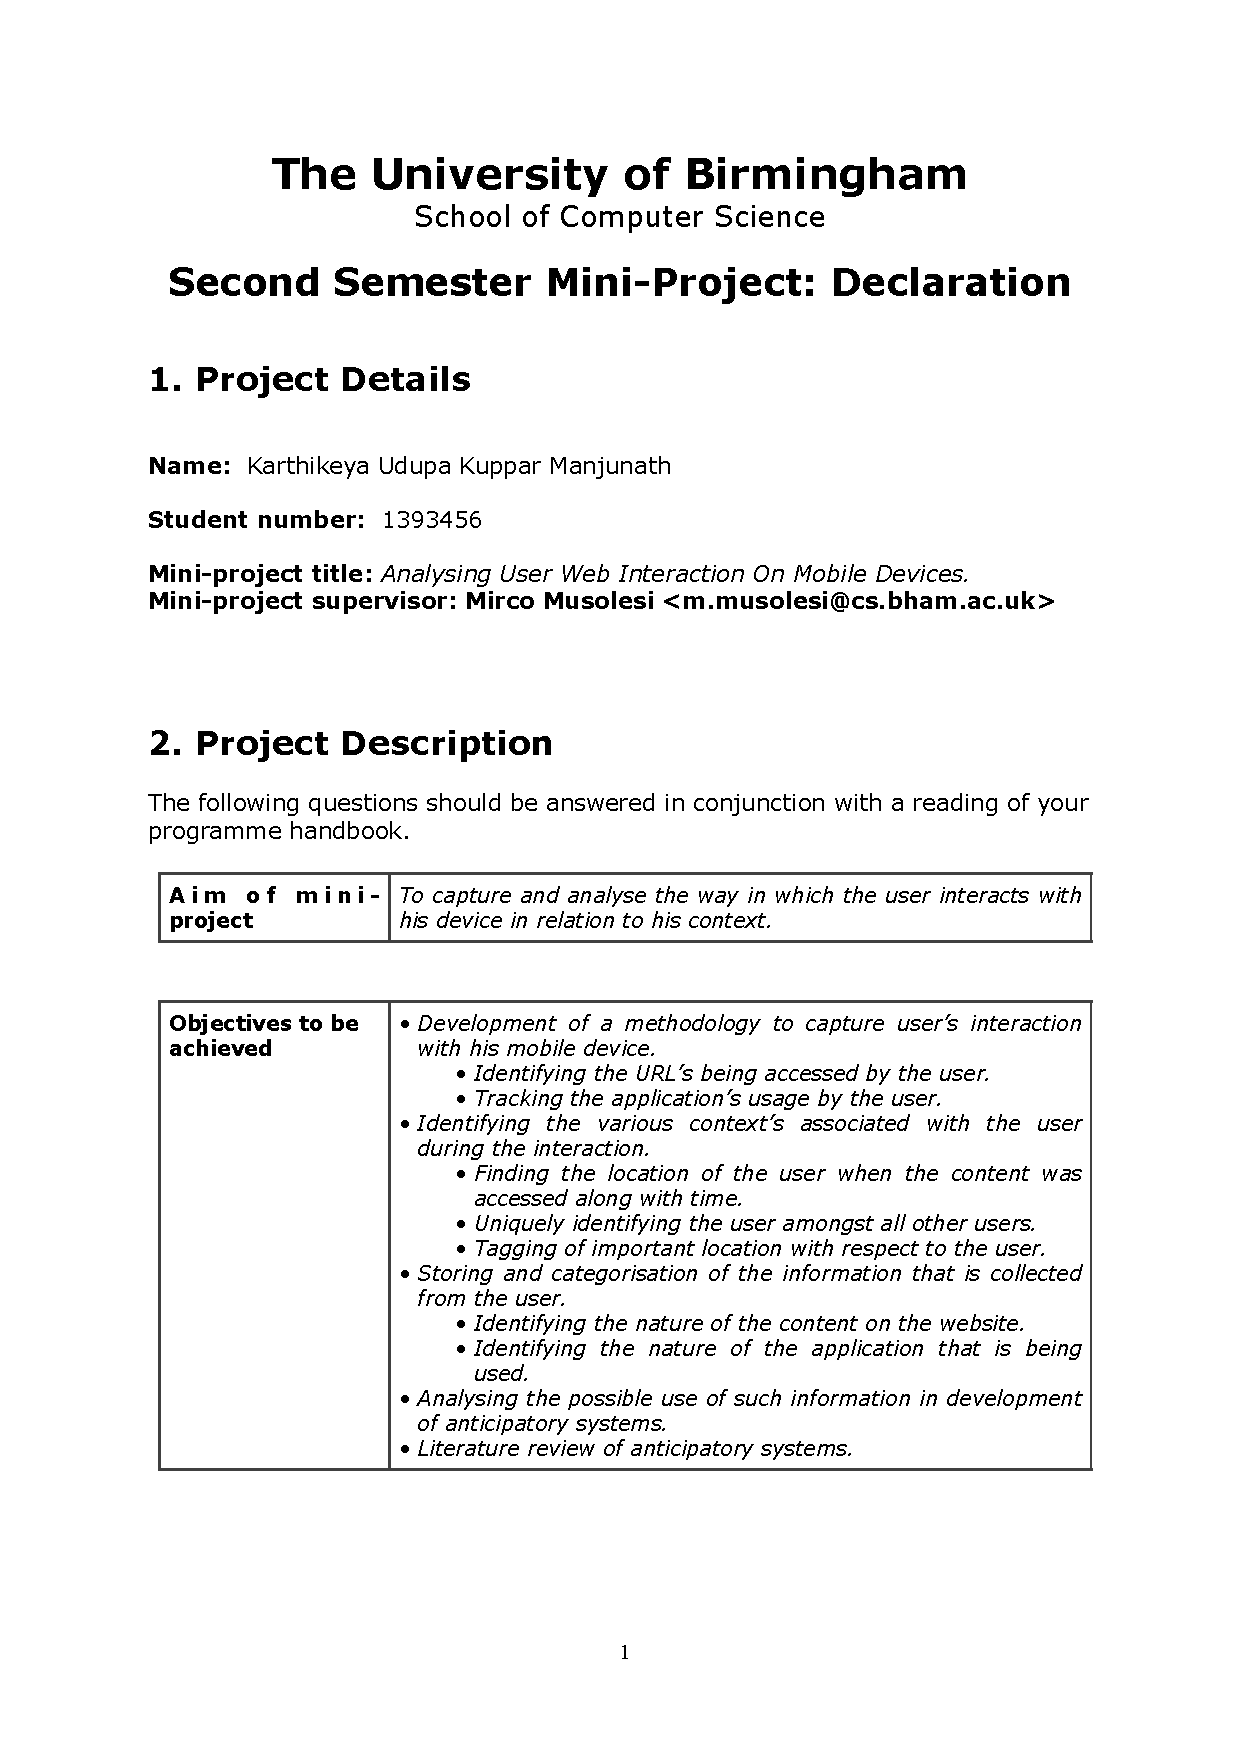
\includepdf[pages={1,2}]{Declaration.pdf}

\chapter{Statement of information search strategy}

statement of search
\end{document}